\chapter{Desarrollo con IA}

\section{Metodología de desarrollo con agentes}

\subsection{Metodología general}

El proyecto se desarrolló con una metodología apoyada en agentes de
programación. Codex y Claude Code ejecutaron tareas de implementación,
refactorización, pruebas y documentación. El criterio humano se mantuvo en las
decisiones de arquitectura, alcance, aceptación y validación.

La regla principal fue separar decisiones y ejecución. El equipo humano definía
objetivo, restricciones y evidencia esperada. El agente implementaba dentro de
ese marco. Después se revisaban diffs, tests, logs, artefactos y resultados de
CI. Este flujo sitúa al humano como \textit{human-in-the-loop}: no corrige cada
línea manualmente, pero decide cuándo una salida puede aceptarse.

\begin{table}[H]
\begin{center}
\small
\begin{tabular}{|p{3.1cm}|p{3.8cm}|p{5.2cm}|} \hline
\textbf{Nivel} & \textbf{Responsable} & \textbf{Control aplicado} \\ \hline
Producto y alcance & Humano & Decide qué problema se resuelve y qué queda fuera. \\ \hline
Arquitectura & Humano con apoyo de agentes & Define contratos, límites entre fases y riesgos aceptables. \\ \hline
Implementación & Agente de programación & Escribe código, tests, migraciones, UI o documentación. \\ \hline
Aceptación & Humano y CI & Revisa evidencia, resultados locales, CI y comportamiento observado. \\ \hline
\end{tabular}
\caption{Modelo de colaboración humano-agente.}
\end{center}
\end{table}

Esta metodología también se aplicó al sistema construido. Los agentes de fase 1
producen artefactos, pero las decisiones relevantes pasan por revisión humana
antes de consolidarse en memoria o de registrarse como modelos aceptados.
La Sección~\ref{ap:desarrollo-agentes-extendido} amplía el flujo de trabajo con
Linear, Hydra, agentes trabajadores y revisión de resultados.

\subsection{Planificación y ejecución autónoma}

Las tareas se organizaron en Linear. Cada tarea incluía objetivo, criterios de
aceptación, dependencias y posible solapamiento con otras zonas del repositorio.
Esto permitió lanzar agentes en paralelo sin mezclar cambios incompatibles.

La ejecución más autónoma se hizo con la skill \texttt{hydra}. Hydra actuaba
como orquestador: leía tareas pendientes, agrupaba trabajo no conflictivo,
lanzaba agentes en worktrees separados, revisaba resultados y cerraba o creaba
seguimiento.

\begin{figure}[H]
\centering
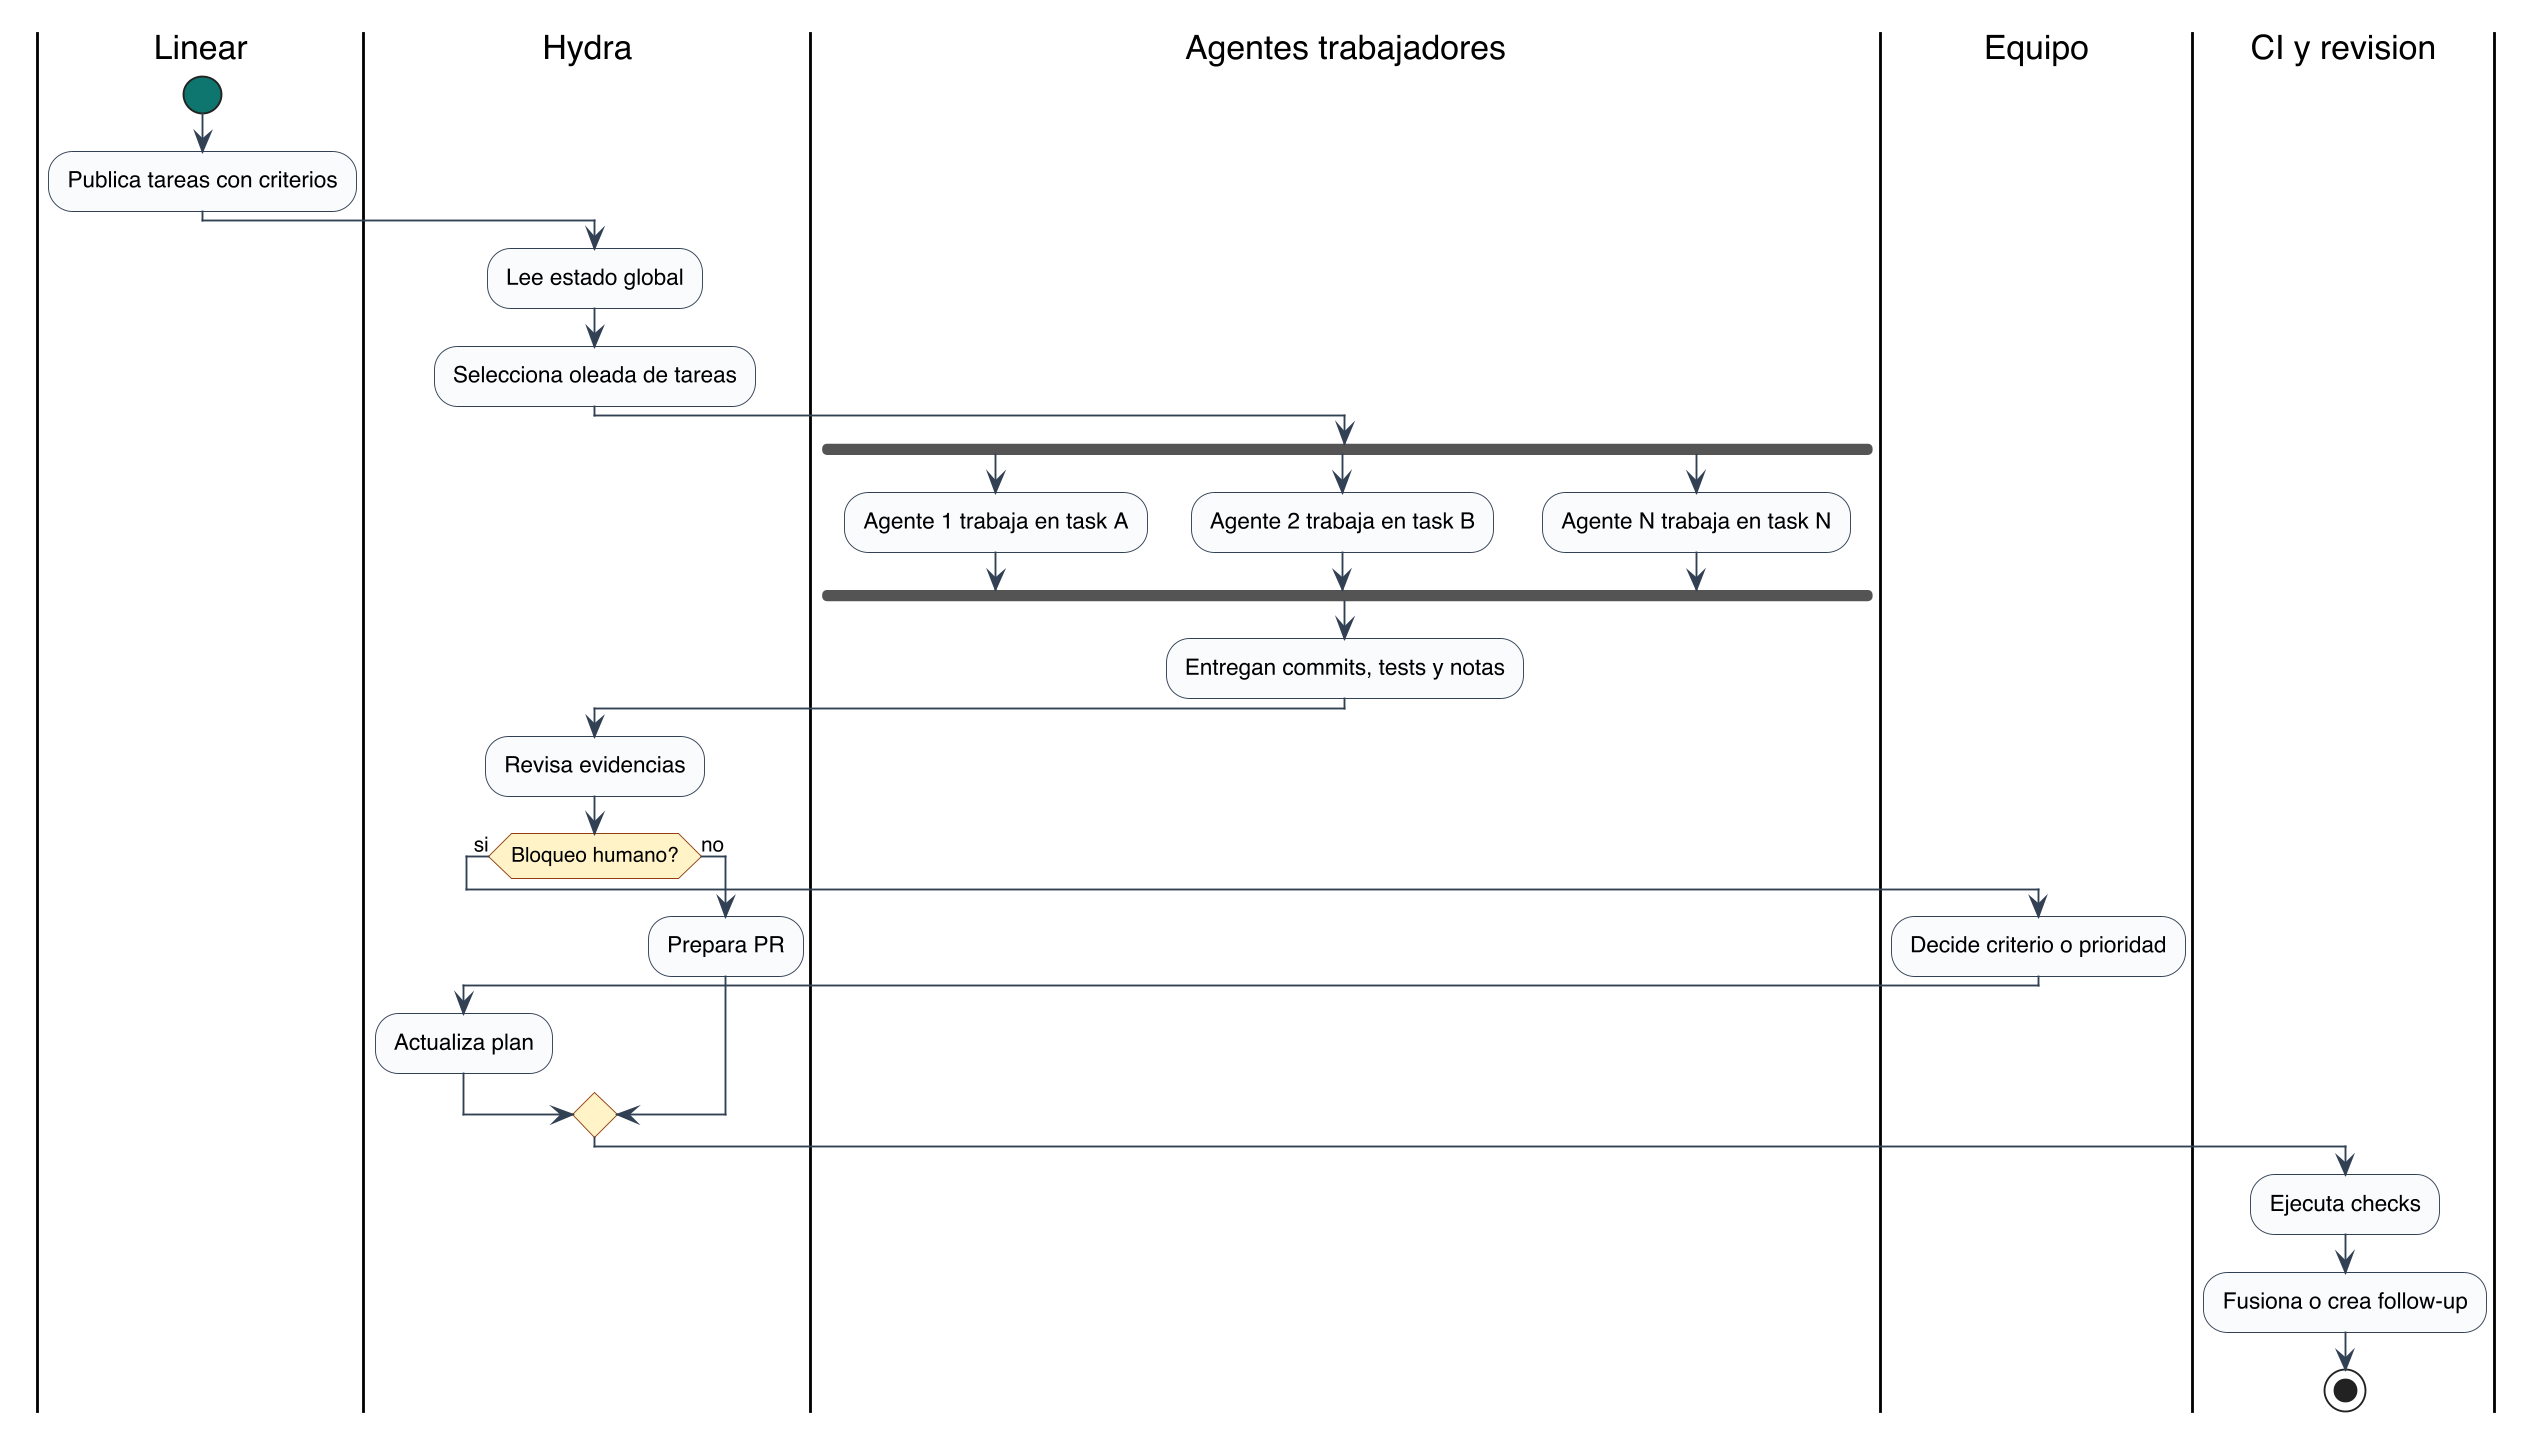
\includegraphics[width=0.86\textwidth,height=0.46\textheight,keepaspectratio]{figuras/phase1-hydra-activity}
\caption{Flujo de orquestación autónoma con Hydra.}
\end{figure}

\subsection{Configuración de agentes}

Los agentes de desarrollo se configuraron mediante instrucciones persistentes,
skills y herramientas. Las skills encapsulan prácticas reutilizables: cómo
trabajar con UI, cómo publicar cambios, cómo revisar CI, cómo usar estilos de
documentación o cómo coordinar agentes.

\begin{table}[H]
\begin{center}
\small
\begin{tabular}{|p{3.1cm}|p{4.4cm}|p{4.8cm}|} \hline
\textbf{Configuración} & \textbf{Uso} & \textbf{Por qué fue necesaria} \\ \hline
Instrucciones del repo & Convenciones de \texttt{uv}, \texttt{pnpm}, commits, estilo y verificación. & Evitan que cada agente reinvente reglas locales. \\ \hline
Skills de desarrollo & UI, GitHub, CI, revisión, documentación y orquestación. & Convierten prácticas repetidas en protocolos reutilizables. \\ \hline
Contexto acotado & Cada agente recibe solo la tarea y los ficheros relevantes. & Reduce ruido y evita degradación por exceso de contexto. \\ \hline
Evidencia obligatoria & Tests, logs, capturas, PDF o CI según la tarea. & Permite aceptar trabajo por pruebas, no por confianza en la respuesta. \\ \hline
\end{tabular}
\caption{Configuración usada para agentes de desarrollo.}
\end{center}
\end{table}

\subsection{Tools, MCP y modelos de lenguaje}

Los agentes usaron herramientas externas para trabajar sobre el repositorio y
los servicios del proyecto. En desarrollo, las herramientas más importantes
fueron shell, Git, GitHub, navegador, Docker, Playwright y editores de ficheros.
Cuando estaban disponibles, los MCPs permitieron operar sobre servicios como
GitHub, Linear o navegación automatizada con una interfaz más estructurada.

\begin{table}[H]
\begin{center}
\small
\begin{tabular}{|p{3.1cm}|p{4.5cm}|p{4.7cm}|} \hline
\textbf{Agente o uso} & \textbf{Modelo o plataforma} & \textbf{Función principal} \\ \hline
Codex & Modelo de programación en entorno terminal & Backend, tests, infraestructura, LaTeX, CI y razonamiento sobre el repo. \\ \hline
Claude Code & Modelo de programación con foco en producto & Frontend, interacción, experiencia de usuario y pulido visual. \\ \hline
Agentes de fase 1 & Modelos vía Anthropic SDK u OpenRouter & Investigación, formalización, adaptación, construcción y memoria. \\ \hline
Juez de evals & LLM externo con rúbrica fija & Revisión separada de artefactos congelados. \\ \hline
\end{tabular}
\caption{Modelos de lenguaje usados por tipo de tarea.}
\end{center}
\end{table}

\section{Decisiones técnicas y tradeoffs}

Las decisiones siguientes fueron las más difíciles porque afectan a la
trazabilidad, coste, escalabilidad y validez científica del sistema.

\begin{table}[H]
\begin{center}
\scriptsize
\begin{tabular}{|p{2.5cm}|p{3.1cm}|p{3.2cm}|p{3.7cm}|} \hline
\textbf{Situación} & \textbf{Decisión tomada} & \textbf{Alternativas} & \textbf{Tradeoffs} \\ \hline
Estado del pipeline & Router determinista con máquina de estados. & Planner libre basado en LLM. & Menos flexibilidad, pero más reanudación, depuración y control humano. \\ \hline
Metadatos y aceptación & PostgreSQL como base relacional. & MongoDB, documentos JSON o solo ficheros. & Más esquema y migraciones, pero consultas fiables sobre runs, modelos, memoria, confianza y validez. \\ \hline
Artefactos grandes & MinIO/S3 para informes, specs, código y trazas. & Guardar blobs en SQL o carpetas locales. & Añade servicio externo, pero evita inflar SQL y permite rutas auditables por run. \\ \hline
Recuperación de memoria & Búsqueda híbrida dense y sparse. & Solo embeddings o solo BM25. & Más coste e infraestructura, pero cubre sinonimia científica y coincidencias exactas de nombres, slugs y variables. \\ \hline
Tamaño de memoria & Grafo, vectores y metadatos separados. & Memoria corta en prompt o un único almacén. & Mayor complejidad, pero permite recuperar hechos, relaciones y procedencia sin saturar contexto. \\ \hline
Escritura de memoria & Solo artefactos aceptados por revisión. & Guardar toda salida del agente. & Menos automatismo, pero evita consolidar alucinaciones o formulaciones rechazadas. \\ \hline
Contrato con fase 2 & Duck typing con \texttt{decide}, \texttt{update} y \texttt{get\_state}. & Clase base común, adaptadores o API remota. & Menos garantías estáticas, pero modelos autocontenidos y bajo acoplamiento entre fases. \\ \hline
Paralelización & Subagentes por paradigma, formulación o spec. & Agente monolítico por ejecución. & Más coordinación, pero fallos aislados y mejor uso de contexto. \\ \hline
Evaluación & Tests, evals YAML y juez LLM separado. & Revisión manual informal o solo unit tests. & Más coste, pero detecta fallos de pipeline, recuperación y fidelidad científica. \\ \hline
\end{tabular}
\caption{Decisiones técnicas y tradeoffs principales.}
\end{center}
\end{table}

\section{Gaps de diseño resueltos}

La colaboración humano-IA fue útil porque los agentes no solo escribieron
código: también hicieron visibles decisiones que no estaban cerradas.

\begin{table}[H]
\begin{center}
\small
\begin{tabular}{|p{3.1cm}|p{4.2cm}|p{5.1cm}|} \hline
\textbf{Gap} & \textbf{Problema detectado} & \textbf{Resolución} \\ \hline
Frontera fase 1/fase 2 & No estaba claro si los modelos debían depender de clases internas del simulador. & Se fijó el contrato \texttt{DecisionModel} por duck typing. \\ \hline
Memoria aceptada & El sistema podía guardar conocimiento útil, pero también errores plausibles. & Se exigió revisión humana antes de escribir memoria persistente. \\ \hline
Specs no implementables & Reasoner podía proponer variables no observables o reglas ambiguas. & Se permitió devolver invalidaciones explícitas y repetir solo la etapa afectada. \\ \hline
\end{tabular}
\caption{Gaps de diseño cerrados durante el desarrollo con IA.}
\end{center}
\end{table}

\section{Reglas de comportamiento de los agentes}

Los criterios de aceptación se redactaron como reglas operativas para agentes de
desarrollo y agentes del sistema.

\begin{table}[H]
\begin{center}
\small
\begin{tabular}{|p{3.2cm}|p{5.1cm}|p{4.1cm}|} \hline
\textbf{Regla} & \textbf{Comportamiento esperado} & \textbf{Evidencia} \\ \hline
Persistir antes de avanzar & Cada etapa guarda artefactos y estado. & MinIO, PostgreSQL y trazas. \\ \hline
No inventar observables & Reasoner solo usa acciones y percepciones del entorno. & Validación de spec o invalidación explícita. \\ \hline
Probar código generado & Builder crea y ejecuta tests. & Resultado de \texttt{pytest}. \\ \hline
No consolidar borradores & MemoryAgent escribe solo artefactos aceptados. & Registro de revisión y memoria. \\ \hline
Devolver errores estructurados & Herramientas y agentes comunican fallos revisables. & Logs, JSON de validación y reportes. \\ \hline
\end{tabular}
\caption{Reglas de comportamiento de los agentes.}
\end{center}
\end{table}

\section{Componentes implementados y tecnologías}

\begin{table}[H]
\begin{center}
\scriptsize
\begin{tabular}{|p{2.7cm}|p{4.6cm}|p{5.1cm}|} \hline
\textbf{Componente} & \textbf{Tecnologías} & \textbf{Uso} \\ \hline
Interfaz web & React, Vite, Tailwind CSS, \texttt{@ppazosp/agrex} & Seguimiento, revisión humana y reproducción de trazas. \\ \hline
API de fase 1 & FastAPI, WebSocket, Uvicorn & Servidor del pipeline y comunicación en tiempo real. \\ \hline
CLI y Router & Typer, Rich, Questionary, \texttt{agrex} & Ejecuciones locales, máquina de estados y traza estructurada. \\ \hline
Agentes & Anthropic SDK, OpenRouter, Pydantic & Llamadas LLM, herramientas y validación de salidas. \\ \hline
Búsqueda & DDGS, búsqueda académica, corpus de evaluación & Fuentes para Researcher y DeepResearcher. \\ \hline
Artefactos & MinIO, API S3, \texttt{aioboto3} & Informes, specs, código, tests, estado y trazas. \\ \hline
Persistencia & PostgreSQL, SQLAlchemy async, asyncpg, Alembic & Runs, modelos, memoria y auditoría. \\ \hline
Memoria & Neo4j, Qdrant, Voyage AI, ZeroEntropy, BM25 & Grafo, recuperación densa, recuperación léxica y reranking. \\ \hline
Validación & uv, pytest, GitHub Actions & Tests de modelos, unit tests, lint y formato. \\ \hline
\end{tabular}
\caption{Componentes software y tecnologías de implementación.}
\label{tab:componentes-tecnologias}
\end{center}
\end{table}

\section{Resultado de la interfaz web}

Como evidencia del resultado implementado, se restauró en local el paquete de
artefactos de CASO1 usado en la evaluación de corpus cerrado de la
Sección~\ref{sec:evaluacion-corpus-cerrado}. La Figura~\ref{fig:phase1-ui-replay-run}
muestra la interfaz final sobre una ejecución real, no un diseño inicial.

\begin{figure}[H]
\centering
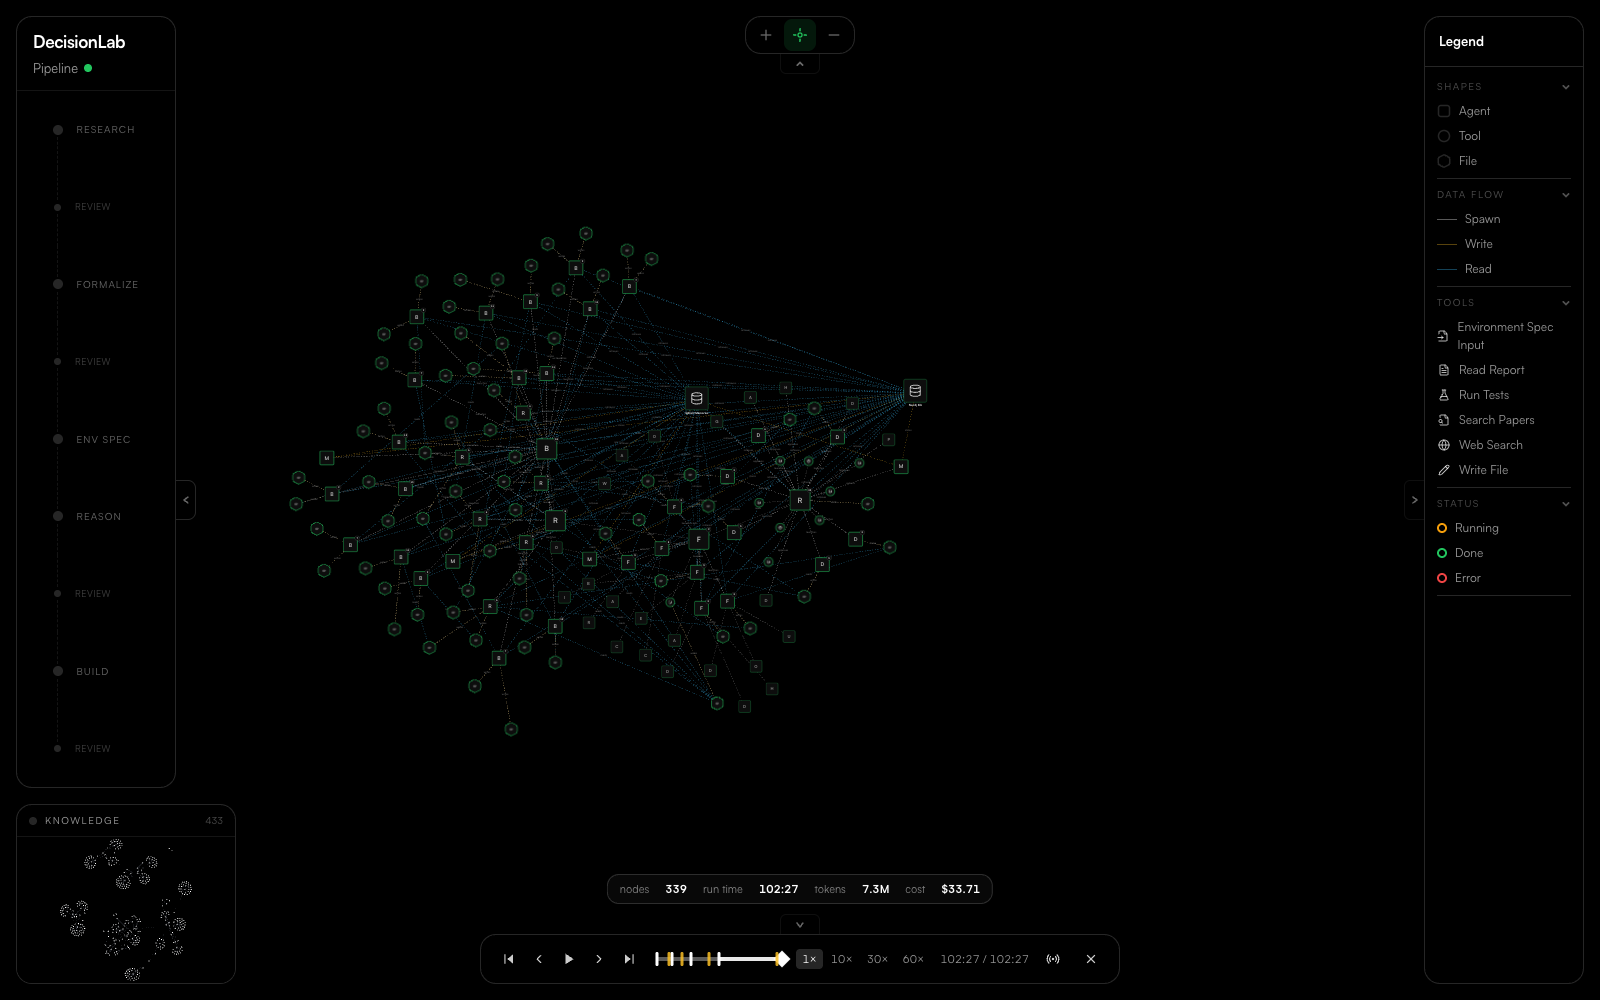
\includegraphics[width=0.86\textwidth,height=0.34\textheight,keepaspectratio]{figuras/phase1-ui-replay-run}
\caption{Interfaz web reproduciendo la ejecución CASO1 restaurada.}
\label{fig:phase1-ui-replay-run}
\end{figure}
